% Software Engineering & System Simulation
% Interview deck for Delta Electronics software roles and NVIDIA software /
% system-software roles. November 6, 2026.
%
% Engine: pdfLaTeX (same as NV-Testing). 16:9 Beamer.
% Diagrams are TikZ in this file. Do not add measured results, incidents,
% or a claim that the LLM simulator is already integrated.
%
% Facts reused from the reference decks:
%   NV-Testing           -- NeoPower platform components and reliability workflow
%   Mapping-HBF-Project  -- custom simulator; HBF is modeled, not measured
%
% Slide sequence:
%  1 Cover
%  2 NeoPower architecture
%  3 NeoPower scenario simulation
%  4 NeoPower testing and reliability
%  5 Bridge
%  6 Heterogeneous GPU / memory design space
%  7 Proposed serving-simulation method
%  8 Progress and roadmap
%  9 Thank you

\documentclass[aspectratio=169,10pt]{beamer}
\usepackage[english]{babel}
\usepackage[utf8]{inputenc}
\usepackage[T1]{fontenc}
\usepackage{lmodern}
\usepackage{amsmath,amssymb}
\usepackage{graphicx}
\usepackage{xcolor}
\usepackage{tikz}
\usetikzlibrary{arrows.meta,positioning,calc,fit,backgrounds}
\usepackage{hyperref}
\graphicspath{{./}{figures/}}
\hypersetup{hidelinks}

% --------- Madrid-inspired identity, matched to NV-Testing ---------
\usetheme{Madrid}
\usecolortheme{default}
\definecolor{Ink}{HTML}{243748}
\definecolor{Muted}{HTML}{667B8B}
\definecolor{Accent}{HTML}{347E74}
\definecolor{AccentBlue}{HTML}{507DAD}
\definecolor{SoftMint}{HTML}{E6F4EE}
\definecolor{SoftBlue}{HTML}{E9F2F9}
\definecolor{SoftLilac}{HTML}{F1EEF8}
\definecolor{Paper}{HTML}{FBFCFE}
\definecolor{Divider}{HTML}{D8E4EB}
\setbeamercolor{background canvas}{bg=Paper}
\setbeamercolor{normal text}{fg=Ink}
\setbeamercolor{structure}{fg=Accent}
\setbeamercolor{frametitle}{fg=Ink,bg=SoftBlue}
\setbeamercolor{title}{fg=Ink}
\setbeamercolor{subtitle}{fg=Muted}
\setbeamercolor{block title}{fg=Ink,bg=SoftBlue}
\setbeamercolor{block body}{fg=Ink,bg=white}
\setbeamercolor{item}{fg=Accent}
\setbeamercolor{footline}{fg=Muted,bg=Paper}
\setbeamercolor{panelblue}{fg=Ink,bg=SoftBlue!60}
\setbeamercolor{panelmint}{fg=Ink,bg=SoftMint!72}
\setbeamercolor{panellilac}{fg=Ink,bg=SoftLilac!76}
\setbeamercolor{panelwhite}{fg=Ink,bg=white}
\setbeamerfont{frametitle}{size=\Large,series=\bfseries}
\setbeamerfont{footline}{size=\tiny}
\setbeamertemplate{headline}{}
\setbeamertemplate{navigation symbols}{}
\setbeamertemplate{blocks}[rounded][shadow=false]
\setbeamertemplate{itemize items}[circle]
\setbeamertemplate{footline}{%
  \leavevmode\hbox{%
    \begin{beamercolorbox}[wd=\paperwidth,ht=.30cm,dp=.16cm,rightskip=.60cm plus 1fil]{footline}%
      \hfill\insertframenumber\,/\,\inserttotalframenumber
    \end{beamercolorbox}}%
}
\setbeamertemplate{frametitle}{%
  \nointerlineskip
  \begin{beamercolorbox}[wd=\paperwidth,ht=.77cm,dp=.18cm,leftskip=.64cm]{frametitle}%
    \usebeamerfont{frametitle}\insertframetitle
  \end{beamercolorbox}%
}

% --------- Reusable text components ---------
\newcommand{\smalllabel}[1]{{\scriptsize\bfseries\color{Accent}\MakeUppercase{#1}}}
\newcommand{\takeaway}[1]{%
  \begin{beamercolorbox}[rounded=true,sep=0.12cm,wd=\linewidth]{block title}%
    \raggedright\strut\textbf{#1}\strut
  \end{beamercolorbox}%
}
\newcommand{\minibadge}[2]{%
  \tikz[baseline=(badge.base)]\node[fill=#1,rounded corners=3pt,
    inner xsep=6pt,inner ysep=3pt] (badge) {\scriptsize\bfseries #2};%
}
\newcommand{\softpanel}[3]{%
  \begin{beamercolorbox}[rounded=true,sep=0.14cm,wd=\linewidth]{#1}%
    \raggedright
    {\small\bfseries\color{Accent}#2}\par\vspace{0.07cm}
    {\small\color{Ink}#3}%
  \end{beamercolorbox}%
}
\newcommand{\smallpanel}[3]{%
  \begin{beamercolorbox}[rounded=true,sep=0.12cm,wd=\linewidth]{#1}%
    \raggedright
    {\small\bfseries\color{Accent}#2}\par\vspace{0.05cm}
    {\scriptsize\color{Ink}#3}%
  \end{beamercolorbox}%
}

% Diagram styles. HBM is blue, HBF is mint, hybrid cells are split.
% Hybrid cell geometry must match memcell: text width 2.48cm, inner sep 3pt,
% minimum height 1.26cm.
\newcommand{\hybridcell}[3]{%
  \begin{scope}
    \clip[rounded corners=3pt] (#1-1.35,#2-0.63) rectangle (#1+1.35,#2+0.63);
    \fill[SoftBlue!88] (#1-1.35,#2-0.63) rectangle (#1,#2+0.63);
    \fill[SoftMint] (#1,#2-0.63) rectangle (#1+1.35,#2+0.63);
  \end{scope}
  \draw[Ink!30, rounded corners=3pt, line width=0.7pt]
    (#1-1.35,#2-0.63) rectangle (#1+1.35,#2+0.63);
  \node[align=center, font=\scriptsize, text width=2.30cm] at (#1,#2) {#3};
}
\tikzset{
  svc/.style={rounded corners=3pt, align=center, font=\scriptsize,
    inner sep=3.5pt, line width=0.75pt},
  fe/.style={svc, draw=AccentBlue!65, fill=SoftBlue!75,
    text width=2.45cm, minimum height=1.08cm},
  be/.style={svc, draw=Accent!80, fill=SoftMint,
    text width=3.35cm, minimum height=1.08cm},
  store/.style={svc, draw=AccentBlue!45, fill=white,
    text width=2.55cm, minimum height=1.28cm},
  extbox/.style={svc, draw=AccentBlue!55, fill=SoftLilac,
    text width=2.75cm, minimum height=1.08cm},
  scen/.style={rounded corners=3pt, align=center, font=\scriptsize,
    text width=2.85cm, minimum height=2.02cm, inner sep=3.5pt, line width=0.75pt,
    execute at begin node={\hyphenpenalty=10000\exhyphenpenalty=10000\sloppy}},
  flowstep/.style={draw=Accent!65, fill=white, rounded corners=3pt,
    minimum height=0.92cm, text width=2.20cm, align=center,
    inner sep=3pt, font=\scriptsize, line width=0.75pt},
  memcell/.style={rounded corners=3pt, align=center, font=\scriptsize,
    text width=2.48cm, minimum height=1.26cm, inner sep=3pt, line width=0.7pt},
  demand/.style={rounded corners=3pt, align=center, font=\scriptsize,
    text width=3.05cm, minimum height=0.68cm, inner sep=2pt, line width=0.7pt},
  srcbox/.style={rounded corners=3pt, align=flush left, font=\scriptsize,
    text width=3.25cm, minimum height=1.78cm, inner sep=4pt, line width=0.75pt},
  hubbox/.style={rounded corners=3pt, align=flush left, font=\scriptsize,
    text width=3.85cm, minimum height=3.72cm, inner sep=5pt, line width=0.8pt},
  method/.style={rounded corners=3pt, align=center, font=\scriptsize\bfseries,
    minimum height=0.72cm, text width=2.85cm, inner sep=3pt}
}

\title[Software Engineering]{Software Engineering \& System Simulation}
\subtitle{Production Backend Development / GPU LLM Serving Research}
\author{Yu-Jui Liang}
\institute{National Taiwan University}
\date{November 6, 2026}

\begin{document}

% ============================================================
% SLIDE 1 - Cover
% ============================================================
{\setbeamertemplate{footline}{}
\begin{frame}[plain]
  \vspace*{0.82cm}
  \smalllabel{Software Engineer Interview}\par
  \vspace{0.48cm}
  {\raggedright\fontsize{18}{22}\selectfont\bfseries\color{Ink}
    Software Engineering \& System Simulation\par}
  \vspace{0.34cm}
  {\color{Muted}\normalsize Production Backend Development \quad$\cdot$\quad GPU LLM Serving Research\par}
  \vspace{0.72cm}
  {\bfseries Yu-Jui Liang}\par
  \vspace{0.08cm}
  {\normalsize\color{Muted}M.S.\ in Data Science\par}
  \vspace{0.04cm}
  {\small\color{Muted}National Taiwan University \quad|\quad Expected Graduation: June 2027\par}
  \vspace{0.03cm}
  {\small\color{Muted}November 6, 2026\par}
  \vfill
  {\color{Accent}\rule{\textwidth}{0.7pt}}\par\vspace{0.08cm}
  {\small\bfseries\color{Muted}Backend Integration \quad/\quad System Simulation \quad/\quad Performance Evaluation}
\end{frame}}

% ============================================================
% SLIDE 2 - NeoPower architecture
% Personal scope: backend integration and debugging in an existing platform.
% Do not describe every box as personally designed.
% ============================================================
\begin{frame}{NeoPower: Backend System Architecture}
  \vspace{0.01cm}
  \smalllabel{01 / Production Platform}\par\vspace{0.08cm}
  \takeaway{Backend integration and debugging inside a production EV charging platform.}
  \vspace{0.04cm}
  {\centering
  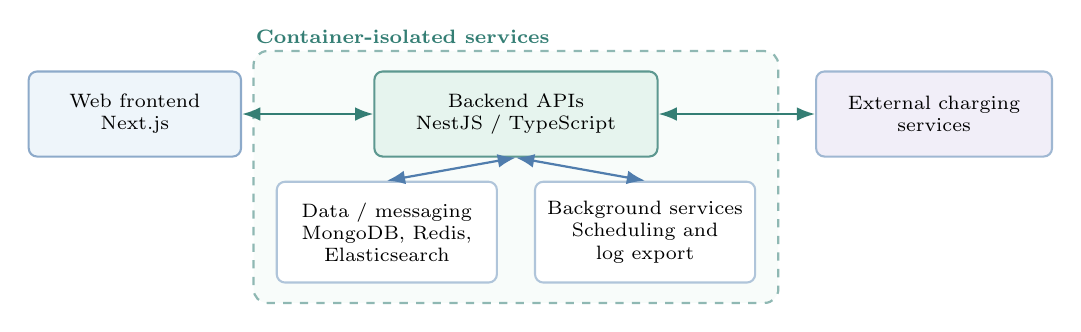
\begin{tikzpicture}[>=Latex]
    % Coordinates keep the external service outside the deployment boundary.
    \node[fe] (ui) at (0,0) {Web frontend\\Next.js};
    \node[be] (api) at (4.84,0) {Backend APIs\\NestJS / TypeScript};
    \node[extbox] (cpo) at (10.15,0) {External charging\\services};
    \node[store] (db) at (3.20,-1.50)
      {Data / messaging\\MongoDB, Redis,\\Elasticsearch};
    \node[store] (jobs) at (6.48,-1.50)
      {Background services\\Scheduling and\\log export};

    \begin{scope}[on background layer]
      \node[draw=Accent!55, dashed, fill=SoftMint!28, rounded corners=5pt,
        line width=0.8pt, inner xsep=8pt, inner ysep=7pt,
        fit={(api)(db)(jobs)}] (boundary) {};
    \end{scope}
    \node[anchor=south west, font=\scriptsize\bfseries, text=Accent, inner sep=1pt]
      at ([yshift=1pt]boundary.north west) {Container-isolated services};

    \draw[<->, Accent, thick] (ui.east) -- (api.west);
    \draw[<->, Accent, thick] (api.east) -- (cpo.west);
    \draw[<->, AccentBlue, thick] (api.south) -- (db.north);
    \draw[<->, AccentBlue, thick] (api.south) -- (jobs.north);
  \end{tikzpicture}\par}
  \vspace{0.06cm}
  \begin{columns}[T,onlytextwidth]
    \begin{column}{0.486\textwidth}
      \smallpanel{panelblue}{Backend / API Integration}{%
        Developing and integrating services within an existing production system.}
    \end{column}
    \begin{column}{0.486\textwidth}
      \smallpanel{panelmint}{Container-Based Service Isolation}{%
        Separating services to support maintenance, deployment, and troubleshooting.}
    \end{column}
  \end{columns}
\end{frame}

% ============================================================
% SLIDE 3 - Scenario simulation
% Supported scope: a custom simulator plus external vendor/client simulators.
% No protocol names, incident stories, or load numbers.
% ============================================================
\begin{frame}{NeoPower: Scenario-Based System Simulation}
  \vspace{0.01cm}
  \smalllabel{02 / Why Simulate}\par\vspace{0.08cm}
  \takeaway{Scenarios reproduce charger and vendor behavior when live equipment cannot.}
  \vspace{0.08cm}
  \begin{center}
  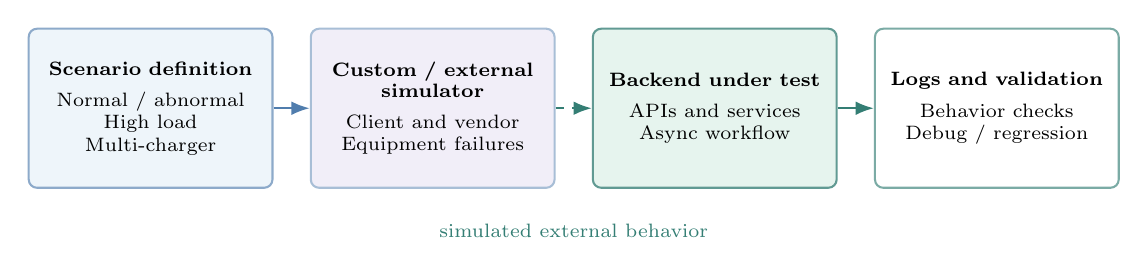
\begin{tikzpicture}[>=Latex, node distance=0.46cm]
    \node[scen, draw=AccentBlue!65, fill=SoftBlue!78] (def)
      {{\bfseries Scenario definition}\\[1.2mm]
       Normal / abnormal\\
       High load\\
       Multi-charger};
    \node[scen, draw=AccentBlue!50, fill=SoftLilac, right=of def] (sim)
      {{\bfseries Custom / external}\\[-0.2mm]
       {\bfseries simulator}\\[1.1mm]
       Client and vendor\\
       Equipment failures};
    \node[scen, draw=Accent!78, fill=SoftMint, right=of sim] (sut)
      {{\bfseries Backend under test}\\[1.2mm]
       APIs and services\\
       Async workflow};
    \node[scen, draw=Accent!65, fill=white, right=of sut] (val)
      {{\bfseries Logs and validation}\\[1.2mm]
       Behavior checks\\
       Debug / regression};
    \draw[->, AccentBlue, thick] (def) -- (sim);
    \draw[->, Accent, thick, dashed] (sim) -- (sut);
    \draw[->, Accent, thick] (sut) -- (val);
    \node[font=\scriptsize, text=Accent, anchor=north] at
      ($(sim.south)!0.5!(sut.south)+(0,-0.32)$)
      {simulated external behavior};
  \end{tikzpicture}
  \end{center}
  \vspace{0.02cm}
  \begin{columns}[T,onlytextwidth]
    \begin{column}{0.32\textwidth}
      \smallpanel{panelblue}{Reproducible workflows}{%
        Re-run a defined scenario without the physical charger or live vendor system.}
    \end{column}
    \begin{column}{0.32\textwidth}
      \smallpanel{panellilac}{Failure and load}{%
        Exercise normal, abnormal, high-load, and multi-charger situations.}
    \end{column}
    \begin{column}{0.32\textwidth}
      \smallpanel{panelmint}{Debug and regression}{%
        Use logs to investigate bugs and keep past failures from returning.}
    \end{column}
  \end{columns}
\end{frame}

% ============================================================
% SLIDE 4 - Testing and production reliability
% Field comparisons are observational. Do not call them a randomized trial.
% ============================================================
\begin{frame}{NeoPower: Testing \& Production Reliability}
  \vspace{0.01cm}
  \smalllabel{03 / Reliability Loop}\par\vspace{0.08cm}
  \takeaway{Production reliability needs reproducible tests and feedback from real deployments.}
  \vspace{0.10cm}
  \begin{columns}[T,onlytextwidth]
    \begin{column}{0.486\textwidth}
      \softpanel{panelblue}{Pre-Deployment Testing}{%
        \textbullet\ Scenario-based validation\\[1.1mm]
        \textbullet\ Vendor / client simulation\\[1.1mm]
        \textbullet\ Regression testing\\[1.1mm]
        \textbullet\ High-load and multi-charger failures}
    \end{column}
    \begin{column}{0.486\textwidth}
      \softpanel{panelmint}{Post-Deployment Validation}{%
        \textbullet\ Operational log analysis\\[1.1mm]
        \textbullet\ Time-based comparison at the same site\\[1.1mm]
        \textbullet\ Cross-site comparison, similar conditions\\[1.1mm]
        \textbullet\ Software behavior and customer feedback}
    \end{column}
  \end{columns}
  \vspace{0.12cm}
  \begin{center}
  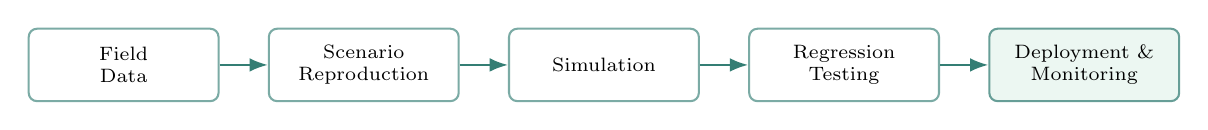
\begin{tikzpicture}[>=Latex]
    \node[flowstep] (a) at (0,0) {Field\\Data};
    \node[flowstep] (b) at (3.05,0) {Scenario\\Reproduction};
    \node[flowstep] (c) at (6.10,0) {Simulation};
    \node[flowstep] (d) at (9.15,0) {Regression\\Testing};
    \node[flowstep, fill=SoftMint!75, draw=Accent!75] (e) at (12.20,0)
      {Deployment \&\\Monitoring};
    \foreach \u/\v in {a/b,b/c,c/d,d/e}{
      \draw[->, thick, Accent] (\u.east) -- (\v.west);
    }
  \end{tikzpicture}
  \end{center}
  \vspace{0.04cm}
  {\scriptsize\color{Muted}Field comparisons are observational checks, not randomized experiments.
  Historical incidents become reusable scenarios for later releases.}
\end{frame}

% ============================================================
% SLIDE 5 - Bridge. Safe to skip in the 5-minute cut.
% ============================================================
\begin{frame}{From Production Systems to GPU Simulation}
  \vspace{0.02cm}
  \smalllabel{04 / Same Engineering Method}\par\vspace{0.08cm}
  \takeaway{Different systems, same loop: model the behavior, then validate it.}
  \vspace{0.16cm}
  \begin{columns}[c,onlytextwidth]
    \begin{column}{0.46\textwidth}
      \begin{beamercolorbox}[rounded=true,sep=0.18cm,wd=\linewidth]{panelmint}
        \raggedright
        {\small\bfseries\color{Accent}NeoPower}\par\vspace{0.10cm}
        {\small Production system simulation for reproducible testing and debugging.}
      \end{beamercolorbox}
    \end{column}
    \begin{column}{0.06\textwidth}
      \centering{\Large\color{Accent}$\rightarrow$}
    \end{column}
    \begin{column}{0.46\textwidth}
      \begin{beamercolorbox}[rounded=true,sep=0.18cm,wd=\linewidth]{panelblue}
        \raggedright
        {\small\bfseries\color{AccentBlue}GPU LLM Serving Research}\par\vspace{0.10cm}
        {\small System-level simulation for evaluating heterogeneous hardware configurations.}
      \end{beamercolorbox}
    \end{column}
  \end{columns}
  \vspace{0.28cm}
  \begin{center}
  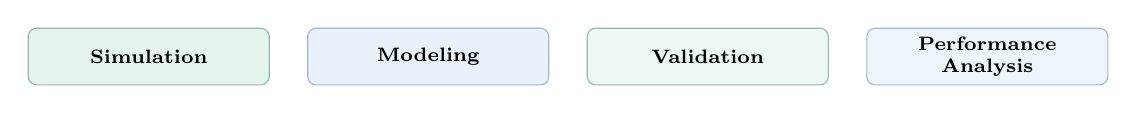
\begin{tikzpicture}
    \node[method, draw=Accent!55, fill=SoftMint] at (0,0) {Simulation};
    \node[method, draw=AccentBlue!55, fill=SoftBlue] at (3.55,0) {Modeling};
    \node[method, draw=Accent!55, fill=SoftMint!70] at (7.10,0) {Validation};
    \node[method, draw=AccentBlue!55, fill=SoftBlue!80] at (10.65,0) {Performance Analysis};
  \end{tikzpicture}
  \end{center}
  \vspace{0.16cm}
  {\scriptsize\color{Muted}Shared method across a production backend and current graduate research.}
\end{frame}

% ============================================================
% SLIDE 6 - Heterogeneous design space
% Six cells are simulation profiles, not six commercial GPUs.
% HBF parameters are not direct hardware measurements.
% ============================================================
\begin{frame}{LLM Serving: Heterogeneous GPU \& Memory}
  \vspace{0.00cm}
  \smalllabel{05 / Graduate Research Question}\par\vspace{0.04cm}
  \takeaway{How should LLM requests be scheduled across GPUs with different compute and memory characteristics?}
  \vspace{0.02cm}
  % Workload demands and the 2 x 3 profile matrix are separate pictures
  % so their coordinates cannot collide. \centering avoids center-env skips.
  {\centering
  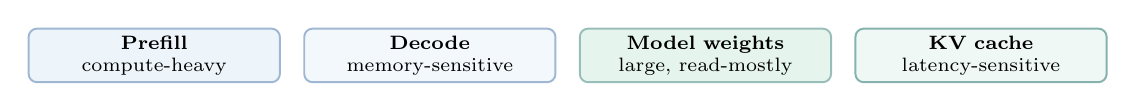
\begin{tikzpicture}
    \node[demand, draw=AccentBlue!55, fill=SoftBlue!80] at (0,0)
      {{\bfseries Prefill}\\compute-heavy};
    \node[demand, draw=AccentBlue!55, fill=SoftBlue!55] at (3.50,0)
      {{\bfseries Decode}\\memory-sensitive};
    \node[demand, draw=Accent!50, fill=SoftMint] at (7.00,0)
      {{\bfseries Model weights}\\large, read-mostly};
    \node[demand, draw=Accent!60, fill=SoftMint!65] at (10.50,0)
      {{\bfseries KV cache}\\latency-sensitive};
  \end{tikzpicture}\par}
  \vspace{0.02cm}
  {\centering
  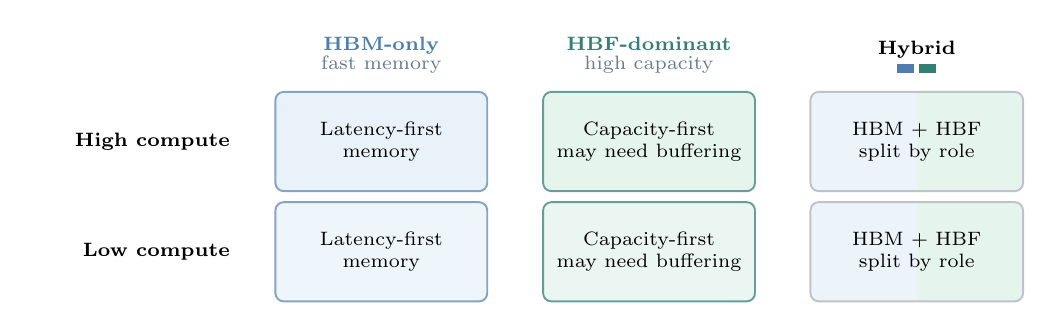
\begin{tikzpicture}
    % Headers sit just above the high-compute row. Blue = HBM, mint = HBF.
    \node[anchor=east, align=right, text width=2.45cm, font=\scriptsize\bfseries]
      at (3.05,0) {High compute};
    \node[anchor=east, align=right, text width=2.45cm, font=\scriptsize\bfseries]
      at (3.05,-1.40) {Low compute};
    \node[anchor=south, align=center, font=\scriptsize] at (4.85,0.74)
      {{\bfseries\color{AccentBlue}HBM-only}\\[-1pt]{\color{Muted}fast memory}};
    \node[anchor=south, align=center, font=\scriptsize] at (8.25,0.74)
      {{\bfseries\color{Accent}HBF-dominant}\\[-1pt]{\color{Muted}high capacity}};
    \node[anchor=south, align=center, font=\scriptsize] at (11.65,0.74)
      {{\bfseries Hybrid}\\[-1pt]%
       {\color{AccentBlue}\rule{0.22cm}{0.12cm}}\hspace{0.06cm}%
       {\color{Accent}\rule{0.22cm}{0.12cm}}};

    \node[memcell, draw=AccentBlue!70, fill=SoftBlue] at (4.85,0)
      {Latency-first\\memory};
    \node[memcell, draw=Accent!75, fill=SoftMint] at (8.25,0)
      {Capacity-first\\may need buffering};
    \node[memcell, draw=AccentBlue!70, fill=SoftBlue!72] at (4.85,-1.40)
      {Latency-first\\memory};
    \node[memcell, draw=Accent!75, fill=SoftMint!78] at (8.25,-1.40)
      {Capacity-first\\may need buffering};
    \hybridcell{11.65}{0}{HBM + HBF\\split by role}
    \hybridcell{11.65}{-1.40}{HBM + HBF\\split by role}
  \end{tikzpicture}\par}
  \vspace{0.01cm}
  \begin{beamercolorbox}[rounded=true,sep=0.045cm,wd=\linewidth]{panelmint}
    \raggedright
    {\scriptsize\bfseries\color{Accent}HBF in this study.}\hspace{0.35em}%
    {\scriptsize Higher capacity, with different latency, bandwidth, power, and endurance.
    The six cells are conceptual simulation profiles, not commercial GPU products.}
  \end{beamercolorbox}
\end{frame}

% ============================================================
% SLIDE 7 - Proposed methodology
% Numbered blocks are the workflow. This system is not implemented yet.
% ============================================================
\begin{frame}{Research Methodology: Simulation Framework}
  \vspace{0.00cm}
  \smalllabel{06 / Proposed Method}\par\vspace{0.07cm}
  \takeaway{Evaluate routing and energy with a system-level serving model.}
  \vspace{0.08cm}
  \begin{center}
  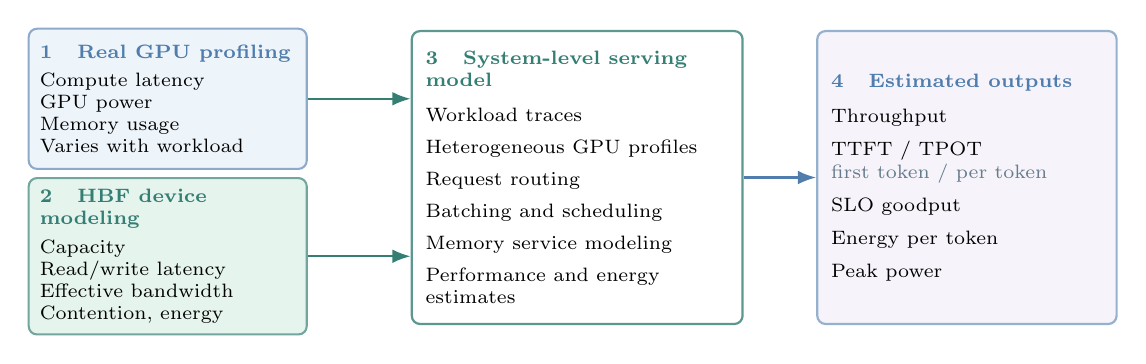
\begin{tikzpicture}[>=Latex]
    \node[srcbox, draw=AccentBlue!65, fill=SoftBlue!75] (gpu) at (0,0.98)
      {{\bfseries\color{AccentBlue}1\quad Real GPU profiling}\\[0.8mm]
       Compute latency\\
       GPU power\\
       Memory usage\\
       Varies with workload};
    \node[srcbox, draw=Accent!70, fill=SoftMint] (hbf) at (0,-1.02)
      {{\bfseries\color{Accent}2\quad HBF device modeling}\\[0.8mm]
       Capacity\\
       Read/write latency\\
       Effective bandwidth\\
       Contention, energy};
    \node[hubbox, draw=Accent!80, fill=white] (sim) at (5.20,-0.02)
      {{\bfseries\color{Accent}3\quad System-level serving model}\\[1.6mm]
       Workload traces\\[1.25mm]
       Heterogeneous GPU profiles\\[1.25mm]
       Request routing\\[1.25mm]
       Batching and scheduling\\[1.25mm]
       Memory service modeling\\[1.25mm]
       Performance and energy estimates};
    \node[hubbox, draw=AccentBlue!60, fill=SoftLilac!65, text width=3.45cm] (out) at (10.15,-0.02)
      {{\bfseries\color{AccentBlue}4\quad Estimated outputs}\\[1.6mm]
       Throughput\\[1.35mm]
       TTFT / TPOT\\[0.2mm]
       {\color{Muted}first token / per token}\\[1.35mm]
       SLO goodput\\[1.35mm]
       Energy per token\\[1.35mm]
       Peak power};
    \draw[->, Accent, thick] (gpu.east) -- (sim.west |- gpu.east);
    \draw[->, Accent, thick] (hbf.east) -- (sim.west |- hbf.east);
    \draw[->, AccentBlue, thick] (sim.east) -- (out.west);
  \end{tikzpicture}
  \end{center}
  \vspace{0.04cm}
  {\scriptsize\color{Muted}Candidates, not yet integrated: LLMServingSim 2.0 and FlashLab HBFSim.
  Scope is system-level behavior, including memory-service contention, not GPU cycle simulation.}
\end{frame}

% ============================================================
% SLIDE 8 - Progress versus plan
% No benchmark numbers and no implemented scheduler.
% ============================================================
\begin{frame}{Current Progress \& Research Roadmap}
  \vspace{0.01cm}
  \smalllabel{07 / Ongoing Research}\par\vspace{0.08cm}
  \takeaway{The question and method are in place. Integration and results are still ahead.}
  \vspace{0.12cm}
  \begin{columns}[T,onlytextwidth]
    \begin{column}{0.486\textwidth}
      \begin{beamercolorbox}[rounded=true,sep=0.16cm,wd=\linewidth]{panelmint}
        \raggedright
        {\small\bfseries\color{Accent}Current Progress}\hfill
        \minibadge{Accent}{\color{white}Completed}\par\vspace{0.12cm}
        {\small\textcolor{Accent}{\checkmark}\hspace{0.35em}Literature survey on heterogeneous GPU serving and HBF memory systems.}\par\vspace{0.12cm}
        {\small\textcolor{Accent}{\checkmark}\hspace{0.35em}Initial formulation of the heterogeneous compute--memory design space.}\par\vspace{0.12cm}
        {\small\textcolor{Accent}{\checkmark}\hspace{0.35em}Evaluation of candidate simulation frameworks and the research method.}
      \end{beamercolorbox}
    \end{column}
    \begin{column}{0.486\textwidth}
      \begin{beamercolorbox}[rounded=true,sep=0.16cm,wd=\linewidth]{panelblue}
        \raggedright
        {\small\bfseries\color{AccentBlue}Next Steps}\hfill
        \minibadge{AccentBlue}{\color{white}Planned}\par\vspace{0.12cm}
        {\small\textcolor{AccentBlue}{$\rightarrow$}\hspace{0.30em}Reproduce LLM serving simulator baselines.}\par\vspace{0.09cm}
        {\small\textcolor{AccentBlue}{$\rightarrow$}\hspace{0.30em}Profile real GPU computation and energy.}\par\vspace{0.09cm}
        {\small\textcolor{AccentBlue}{$\rightarrow$}\hspace{0.30em}Integrate HBM/HBF memory models.}\par\vspace{0.09cm}
        {\small\textcolor{AccentBlue}{$\rightarrow$}\hspace{0.30em}Explore HBF-aware request routing.}\par\vspace{0.09cm}
        {\small\textcolor{AccentBlue}{$\rightarrow$}\hspace{0.30em}Evaluate performance--energy trade-offs under latency SLOs.}
      \end{beamercolorbox}
    \end{column}
  \end{columns}
\end{frame}

% ============================================================
% SLIDE 9 - Close
% ============================================================
{\setbeamertemplate{footline}{}
\begin{frame}[plain]
  \vfill
  \begin{center}
    {\fontsize{38}{44}\selectfont\bfseries\color{Ink}Thank You}\par
    \vspace{0.30cm}
    {\Large\color{Accent}Questions \& Discussion}
  \end{center}
  \vfill
\end{frame}}

\end{document}
